% ============================================================
% BAB 2 - GAMBARAN PRODUK DAN BATAS SISTEM
% ============================================================

\subsection{Product Perspective}

Aplikasi ini menempati posisi sebagai \textbf{Demand Generator B2C} dalam
ekosistem \textit{microservices} UMKM RPL 2. Secara teknis, \textit{frontend}
berjalan di \texttt{pasarkita.vercel.app} (Next.js 16.2) dan \textit{backend}
di \texttt{pasarkita-api.vercel.app} (Express.js \textit{serverless}), keduanya
di-\textit{deploy} terpisah dari repo monorepo yang sama. \textit{Database}
menggunakan Supabase PostgreSQL yang diakses eksklusif oleh \textit{backend}
PasarKita.

Semua komunikasi ke \textit{service} eksternal (SmartBank, LogistiKita) melewati
API Gateway (Kelompok 7) dengan JWT. Untuk keperluan \textit{development} lokal,
tersedia \textit{mock server} di direktori \texttt{mock/} yang mensimulasikan
SmartBank (:4001) dan LogistiKita (:4002).

% Placeholder diagram konteks
\begin{figure}[htbp]
    \centering
    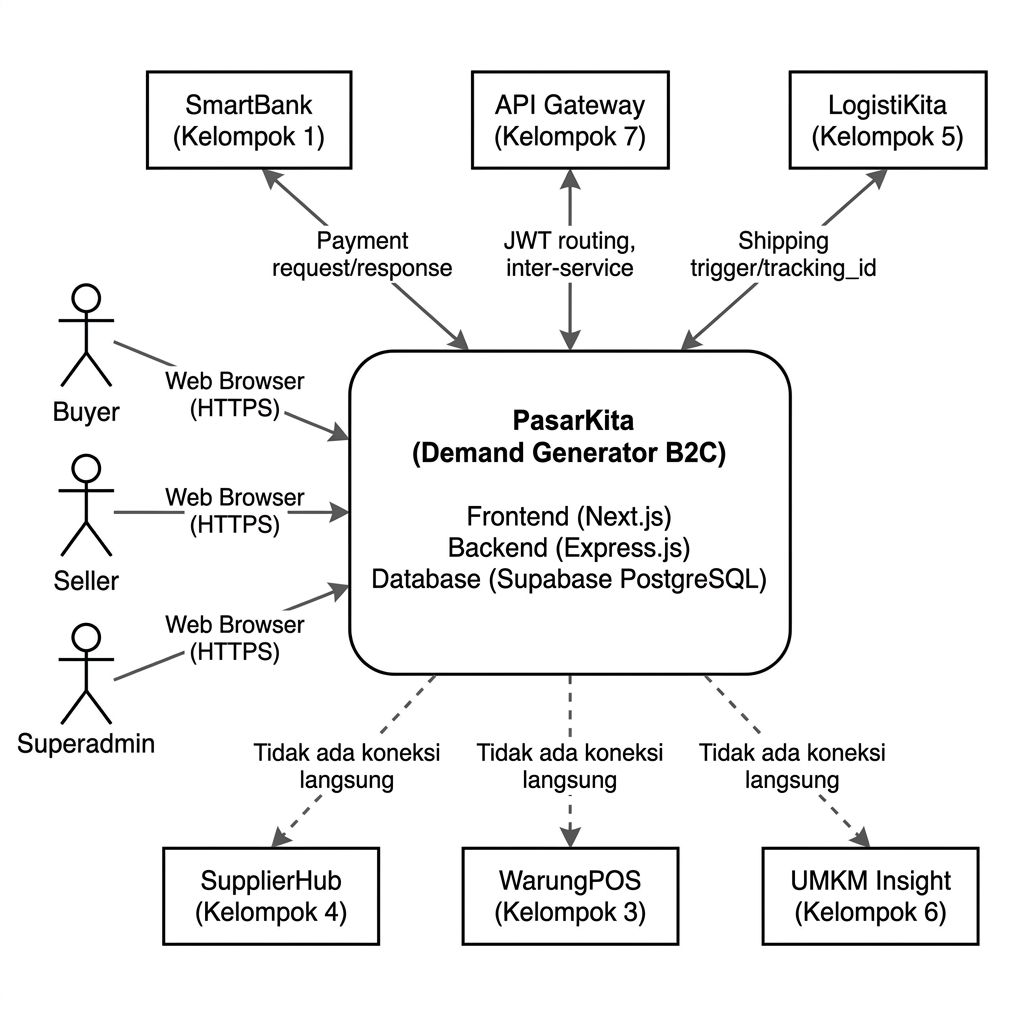
\includegraphics[width=\textwidth]{figures/diagram-konteks.png}
    \caption{Diagram Konteks Sistem PasarKita dalam Ekosistem UMKM RPL 2}
    \label{fig:diagram-konteks}
\end{figure}

% ----
\subsection{User Classes dan Karakteristik}

Sistem melayani beberapa kelas pengguna dengan hak dan ekspektasi yang berbeda.
Kebutuhan sistem harus menjaga perbedaan tersebut agar transaksi
\textit{marketplace} dapat berjalan tanpa mencampuri domain \textit{service} lain
dalam ekosistem.

\begin{longtable}{|L{2.2cm}|L{3.8cm}|L{4.5cm}|L{4cm}|}
    \caption{User Classes dan Karakteristik}
    \label{tab:user-classes} \\
    \hline
    \textbf{User Class} & \textbf{Tanggung Jawab} & \textbf{Ekspektasi Sistem}
        & \textbf{Kontrol Akses} \\
    \hline
    \endfirsthead
    \hline
    \textbf{User Class} & \textbf{Tanggung Jawab} & \textbf{Ekspektasi Sistem}
        & \textbf{Kontrol Akses} \\
    \hline
    \endhead
    \hline
    \endfoot
    Buyer
        & Menelusuri produk, menambahkan ke keranjang, melakukan \textit{checkout},
          memantau status \textit{order}, dan memberikan ulasan.
        & Alur belanja yang mudah, status \textit{order} \textit{real-time},
          konfirmasi pembayaran jelas, riwayat pesanan tersedia.
        & JWT role \texttt{buyer}; tidak dapat mengelola produk atau melihat \textit{analytics}. \\
    \hline
    Seller
        & Mengelola katalog produk sendiri (CRUD), memantau \textit{order} masuk,
          mengelola stok, dan membalas ulasan.
        & \textit{Dashboard} produk yang efisien, notifikasi \textit{order} baru,
          visibilitas stok rendah.
        & JWT role \texttt{seller}; hanya dapat CRUD produk milik sendiri; tidak
          dapat mengakses data \textit{seller} lain. \\
    \hline
    Superadmin
        & Memantau seluruh operasional platform: manajemen \textit{user},
          \textit{order}, \textit{analytics}, moderasi konten, dan \textit{audit log}.
        & \textit{Dashboard analytics} lengkap, kemampuan ban/aktifkan \textit{user},
          \textit{update} status \textit{order} manual, akses \textit{audit log}.
        & JWT role \texttt{superadmin}; dibuat via \textit{insert} manual ke
          Supabase; akses penuh ke semua \textit{endpoint} admin. \\
    \hline
    API Gateway
        & Memvalidasi JWT antar-\textit{service}, meneruskan \textit{payment request}
          ke SmartBank, dan \textit{trigger} ke LogistiKita.
        & Kontrak JSON stabil, \textit{error response} deterministik,
          \textit{idempotency key} pada \textit{checkout}.
        & \textit{Service-to-service} via \textit{header} JWT ekosistem; bukan
          \textit{user} biasa. \\
    \hline
    SmartBank
        & Memproses pembayaran dan mengembalikan \texttt{transaction\_id} atau
          \textit{failure response}.
        & Format \textit{request} konsisten, \textit{idempotency} terjaga,
          \textit{rollback} stok saat pembayaran gagal.
        & Akses melalui API Gateway; tidak ada akses langsung ke \textit{database}
          PasarKita. \\
    \hline
\end{longtable}

% ----
\subsection{Operating Environment}

\begin{longtable}{|L{2.8cm}|L{5.5cm}|L{6.2cm}|}
    \caption{Operating Environment Sistem PasarKita}
    \label{tab:operating-env} \\
    \hline
    \textbf{Komponen} & \textbf{Spesifikasi Saat Ini} & \textbf{Implikasi Requirement} \\
    \hline
    \endfirsthead
    \hline
    \textbf{Komponen} & \textbf{Spesifikasi Saat Ini} & \textbf{Implikasi Requirement} \\
    \hline
    \endhead
    \hline
    \endfoot
    Frontend
        & Next.js 16.2, App Router, TypeScript, Tailwind CSS, shadcn/ui,
          di-\textit{deploy} ke Vercel (\texttt{frontend/}).
        & \textit{Routing} berbasis App Router; komponen UI harus konsisten dengan
          shadcn/ui \textit{design system}. \\
    \hline
    Backend
        & Express.js dengan \texttt{serverless-http}, di-\textit{deploy} ke Vercel
          \textit{serverless function} (\texttt{backend/api/index.js}).
        & Tidak ada \textit{persistent in-memory state}; semua \textit{state} harus
          tersimpan di \textit{database}. \\
    \hline
    Database
        & Supabase PostgreSQL, diakses via Supabase SDK dan \textit{service role key}
          dari \textit{backend}.
        & Skema harus menjaga \texttt{users}, \texttt{products}, \texttt{orders},
          \texttt{order\_items}, \texttt{ratings}, \texttt{notifications},
          \texttt{vouchers}, dan \texttt{audit logs}. \\
    \hline
    State Management
        & Zustand (auth, cart) dan TanStack Query di \textit{frontend}.
        & \textit{Cart state} bersifat \textit{client-side}; sinkronisasi stok
          terjadi saat \textit{checkout} di \textit{backend}. \\
    \hline
    Auth
        & JWT yang di-\textit{generate} \textit{backend} PasarKita saat \textit{login};
          validasi JWT antar-\textit{service} via API Gateway.
        & Token harus menyertakan \textit{role}; \textit{middleware} auth harus
          memvalidasi sebelum setiap \textit{protected route}. \\
    \hline
    Integrasi Ekosistem
        & API Gateway di \texttt{GATEWAY\_BASE\_URL}; SmartBank dan LogistiKita
          diakses via Gateway.
        & Koneksi eksternal harus gagal secara terkendali dan tidak merusak data
          \textit{order} lokal. \\
    \hline
    Mock Server (dev)
        & Express.js lokal di \texttt{mock/smartbank/:4001} dan
          \texttt{mock/logistikita/:4002}.
        & Hanya digunakan saat \texttt{NODE\_ENV=development}; \textit{production}
          selalu melalui \texttt{GATEWAY\_BASE\_URL}. \\
    \hline
    Deploy
        & Dua project Vercel terpisah dari satu repo monorepo (\texttt{frontend/}
          dan \texttt{backend/}).
        & \textit{Environment variables} harus dikonfigurasi terpisah per project
          di Vercel. \\
    \hline
\end{longtable}
